\documentclass[12pt,a4paper]{article}
\usepackage[utf8]{inputenc}
\usepackage[T1]{fontenc}
\usepackage[brazil]{babel}
\usepackage{amsmath,amssymb,amsfonts}
\usepackage{geometry}
\usepackage{graphicx}
\usepackage{float}
\usepackage{booktabs}
\usepackage{siunitx}
\usepackage{xcolor}
\usepackage{listings}
\usepackage{hyperref}
\geometry{left=3cm,right=2cm,top=3cm,bottom=2cm}
\hypersetup{colorlinks=true,allcolors=black}

\lstdefinestyle{pythonstyle}{
    language=Python,
    basicstyle=\ttfamily\small,
    keywordstyle=\color{blue},
    commentstyle=\color{teal!70!black},
    stringstyle=\color{red!60!black},
    numbers=left,
    numberstyle=\tiny,
    stepnumber=1,
    numbersep=8pt,
    showstringspaces=false,
    breaklines=true,
    frame=single,
    tabsize=4
}

\title{Solução Numérica em \LaTeX{} -- Avaliação 1 de Métodos Numéricos}
\author{Gustavo Bittar Gonçalves}
\date{}

\begin{document}
\maketitle

\section{Problema resolvido}
Foi considerada a questão numérica da avaliação, referente à condução de calor bidimensional, transiente, em uma chapa de alumínio puro, com espessura de \SI{5}{mm}, dimensões $L_x=L_y=\SI{1.0}{m}$, condição inicial uniforme $T(x,y,0)=\SI{300}{K}$, e as seguintes condições de contorno:
\begin{itemize}
    \item em $x=0$: temperatura imposta $T=\SI{400}{K}$;
    \item em $x=L_x$: condição adiabática;
    \item em $y=0$: convecção com $h=\SI{100}{W/(m^2.K)}$ e $T_\infty=\SI{350}{K}$;
    \item em $y=L_y$: convecção com $h=\SI{200}{W/(m^2.K)}$, $T_\infty=\SI{280}{K}$, e radiação térmica com $T_{viz}=\SI{300}{K}$ e $\varepsilon=0.8$.
\end{itemize}

Foram adotadas propriedades típicas do alumínio puro: $k=\SI{237}{W/(m.K)}$, $\rho=\SI{2700}{kg/m^3}$ e $c_p=\SI{897}{J/(kg.K)}$, o que fornece
\[
\alpha = \frac{k}{\rho c_p}.
\]

\section{Modelagem matemática}
A equação governante para condução transiente bidimensional com condutividade térmica constante é
\begin{equation}
\frac{\partial T}{\partial t} = \alpha\left(\frac{\partial^2 T}{\partial x^2} + \frac{\partial^2 T}{\partial y^2}\right).
\end{equation}

As condições de contorno ficam:
\begin{align}
T(0,y,t) &= 400, \\
\left.\frac{\partial T}{\partial x}\right|_{x=L_x} &= 0, \\
k\left.\frac{\partial T}{\partial y}\right|_{y=0} &= h_{inf}\left(T-T_{\infty,inf}\right), \\
-k\left.\frac{\partial T}{\partial y}\right|_{y=L_y} &= h_{sup}\left(T-T_{\infty,sup}\right) + \varepsilon\sigma\left(T^4-T_{viz}^4\right).
\end{align}

\section{Discretização numérica}
Foi utilizado:
\begin{itemize}
    \item diferenças finitas centrais de segunda ordem nos termos espaciais;
    \item método de Euler explícito no termo temporal.
\end{itemize}

Para um nó interno $(i,j)$, a discretização é:
\begin{equation}
T_{i,j}^{n+1} = T_{i,j}^{n} + \alpha\Delta t
\left[
\frac{T_{i+1,j}^{n}-2T_{i,j}^{n}+T_{i-1,j}^{n}}{\Delta x^2}
+
\frac{T_{i,j+1}^{n}-2T_{i,j}^{n}+T_{i,j-1}^{n}}{\Delta y^2}
\right].
\end{equation}

\subsection{Tratamento das fronteiras}
\paragraph{Fronteira em $x=0$.}
A condição é de Dirichlet e, portanto, em todo passo de tempo impõe-se diretamente:
\begin{equation}
T_{0,j}^{n+1}=400.
\end{equation}

\paragraph{Fronteira em $x=L_x$.}
A condição adiabática é
\begin{equation}
\left.\frac{\partial T}{\partial x}\right|_{x=L_x}=0.
\end{equation}
Usando nó fantasma com derivada central,
\begin{equation}
\frac{T_g-T_{N_x-2,j}}{2\Delta x}=0 \Rightarrow T_g=T_{N_x-2,j}.
\end{equation}
Logo,
\begin{equation}
\left.\frac{\partial^2 T}{\partial x^2}\right|_{x=L_x}
\approx
\frac{2(T_{N_x-2,j}-T_{N_x-1,j})}{\Delta x^2}.
\end{equation}

\paragraph{Fronteira em $y=0$.}
Na borda inferior:
\begin{equation}
k\left.\frac{\partial T}{\partial y}\right|_{y=0} = h_{inf}(T-T_{\infty,inf}).
\end{equation}
Com nó fantasma,
\begin{equation}
\frac{T_{i,1}-T_g}{2\Delta y}=\frac{h_{inf}}{k}(T_{i,0}-T_{\infty,inf})
\Rightarrow
T_g=T_{i,1}-2\Delta y\frac{h_{inf}}{k}(T_{i,0}-T_{\infty,inf}).
\end{equation}
Substituindo na segunda derivada,
\begin{equation}
\left.\frac{\partial^2 T}{\partial y^2}\right|_{y=0}
\approx
\frac{2(T_{i,1}-T_{i,0})}{\Delta y^2}
-
\frac{2h_{inf}}{k\Delta y}(T_{i,0}-T_{\infty,inf}).
\end{equation}

\paragraph{Fronteira em $y=L_y$.}
Na borda superior:
\begin{equation}
-k\left.\frac{\partial T}{\partial y}\right|_{y=L_y}
=
 h_{sup}(T-T_{\infty,sup}) + \varepsilon\sigma(T^4-T_{viz}^4).
\end{equation}
Com nó fantasma,
\begin{equation}
\frac{T_g-T_{i,N_y-2}}{2\Delta y}
=
-
\frac{1}{k}
\left[
 h_{sup}(T_{i,N_y-1}-T_{\infty,sup}) + \varepsilon\sigma(T_{i,N_y-1}^4-T_{viz}^4)
\right],
\end{equation}
portanto,
\begin{equation}
\left.\frac{\partial^2 T}{\partial y^2}\right|_{y=L_y}
\approx
\frac{2(T_{i,N_y-2}-T_{i,N_y-1})}{\Delta y^2}
-
\frac{2}{k\Delta y}
\left[
 h_{sup}(T_{i,N_y-1}-T_{\infty,sup}) + \varepsilon\sigma(T_{i,N_y-1}^4-T_{viz}^4)
\right].
\end{equation}

\section{Algoritmo numérico}
O algoritmo empregado é:
\begin{enumerate}
    \item definir geometria, propriedades do material e condições de contorno;
    \item escolher a malha $(N_x,N_y)$ e calcular $\Delta x$, $\Delta y$;
    \item calcular um $\Delta t$ estável para Euler explícito;
    \item inicializar todo o domínio com $T=\SI{300}{K}$ e impor $T=\SI{400}{K}$ em $x=0$;
    \item atualizar os nós internos pela equação explícita;
    \item atualizar separadamente as fronteiras usando as expressões deduzidas acima;
    \item repetir até $t=\SI{14400}{s}$;
    \item salvar os campos térmicos, perfis e históricos temporais requeridos.
\end{enumerate}

\section{Observação sobre GPU e fallback}
O programa em Python tenta utilizar \texttt{CuPy} para executar os cálculos em GPU com CUDA, quando disponível. Caso a GPU não esteja disponível, ou o \texttt{CuPy} não esteja instalado, o programa faz \emph{fallback} automático para \texttt{NumPy}, executando em CPU, de forma serial, sem necessidade de alterar o código.

\section{Código Python comentado}
O código completo utilizado está a seguir.

\lstinputlisting[style=pythonstyle]{heat2d_avaliacao_cuda_fallback.py}

\section{Figuras geradas}
O script salva automaticamente as figuras em formato \texttt{PNG}. A seguir estão as referências para inclusão no documento. Basta manter os arquivos na pasta correta ou ajustar os caminhos.

\subsection{Campos de temperatura para a malha $N_x=N_y=10$}
\begin{figure}[H]
    \centering
    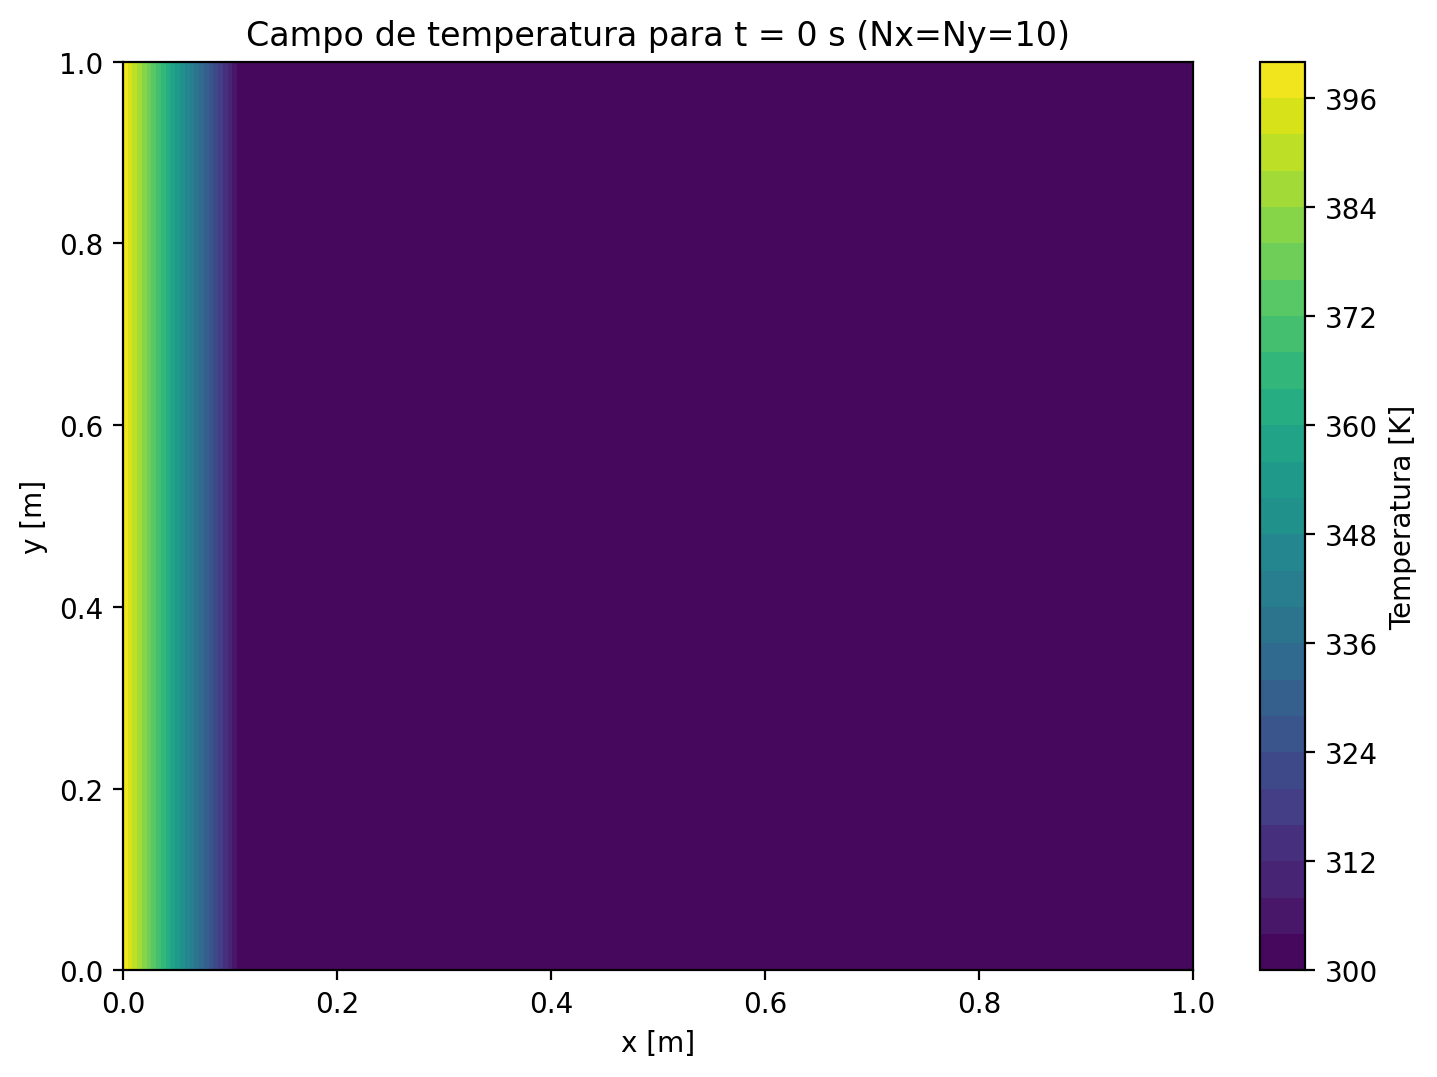
\includegraphics[width=0.75\textwidth]{figuras_avaliacao/campo_temperatura_t_00000.png}
    \caption{Campo de temperatura no instante $t=0\ \text{s}$ para $N_x=N_y=10$.}
    \label{fig:campo_t0}
\end{figure}

\begin{figure}[H]
    \centering
    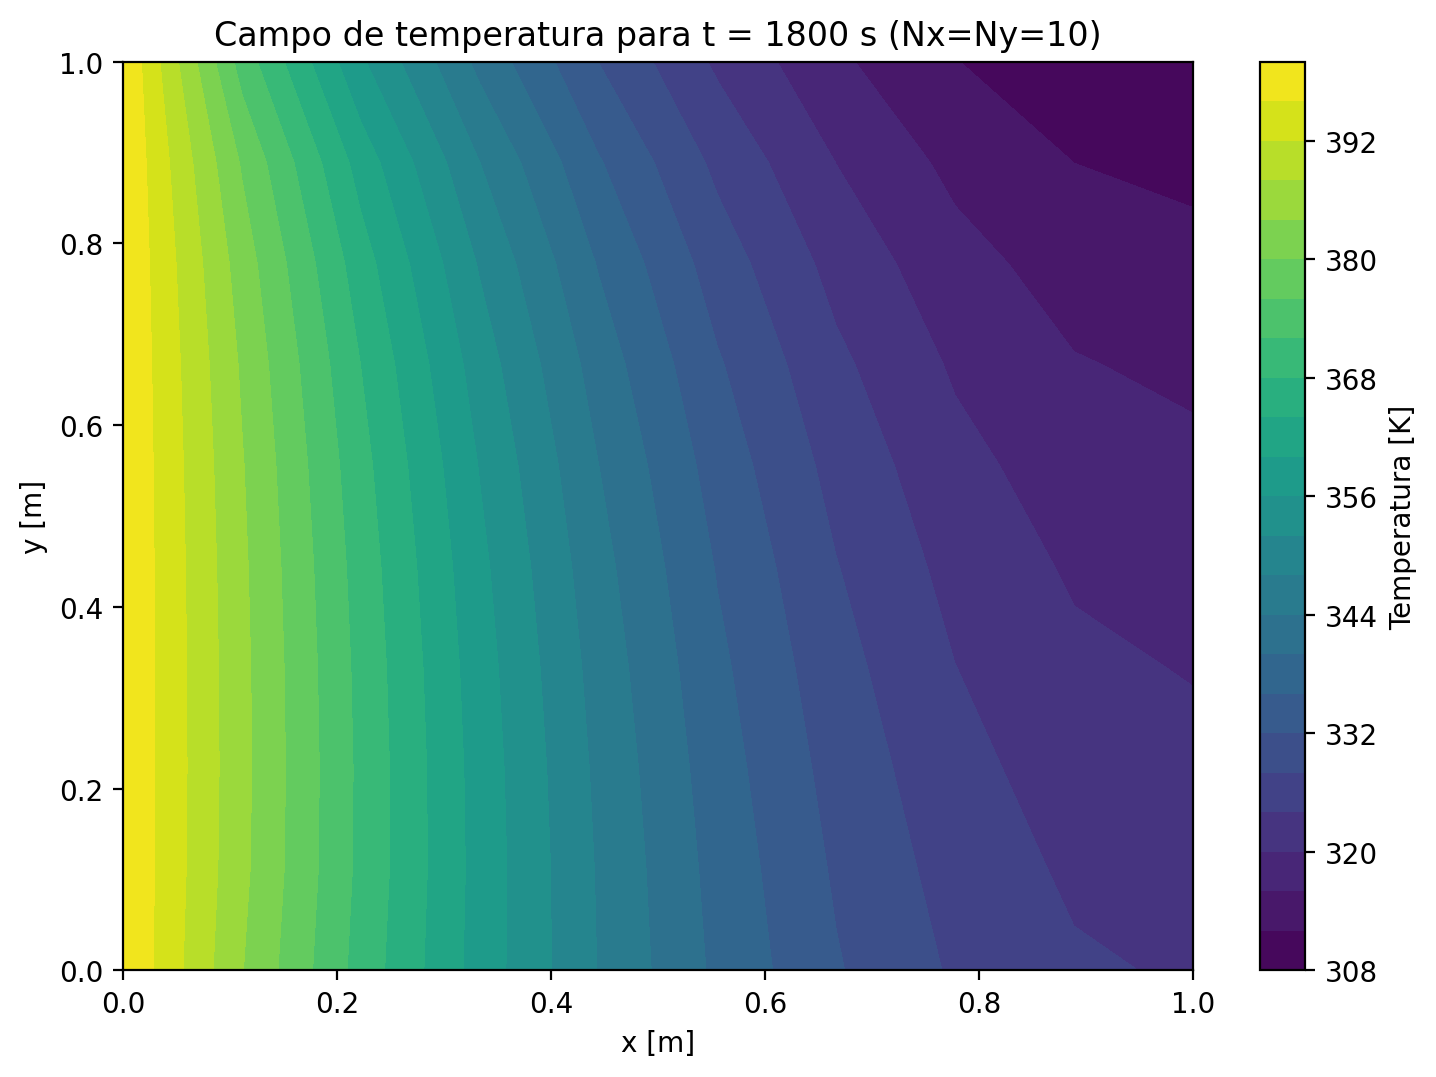
\includegraphics[width=0.75\textwidth]{figuras_avaliacao/campo_temperatura_t_01800.png}
    \caption{Campo de temperatura no instante $t=1800\ \text{s}$ para $N_x=N_y=10$.}
    \label{fig:campo_t1800}
\end{figure}

\begin{figure}[H]
    \centering
    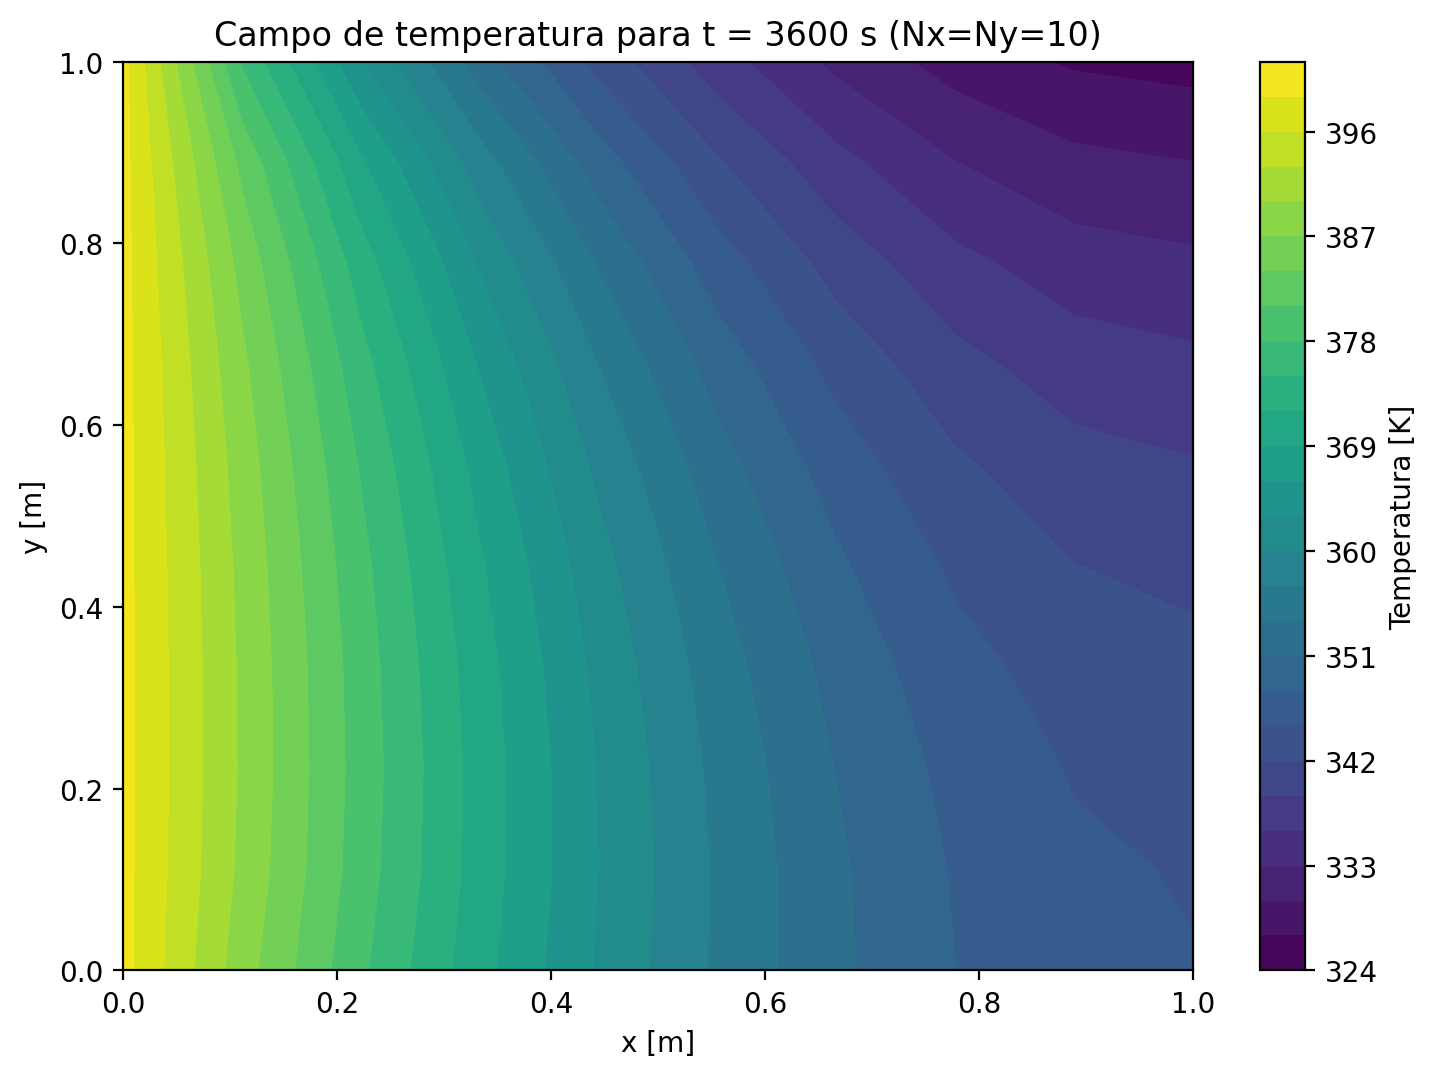
\includegraphics[width=0.75\textwidth]{figuras_avaliacao/campo_temperatura_t_03600.png}
    \caption{Campo de temperatura no instante $t=3600\ \text{s}$ para $N_x=N_y=10$.}
    \label{fig:campo_t3600}
\end{figure}

\begin{figure}[H]
    \centering
    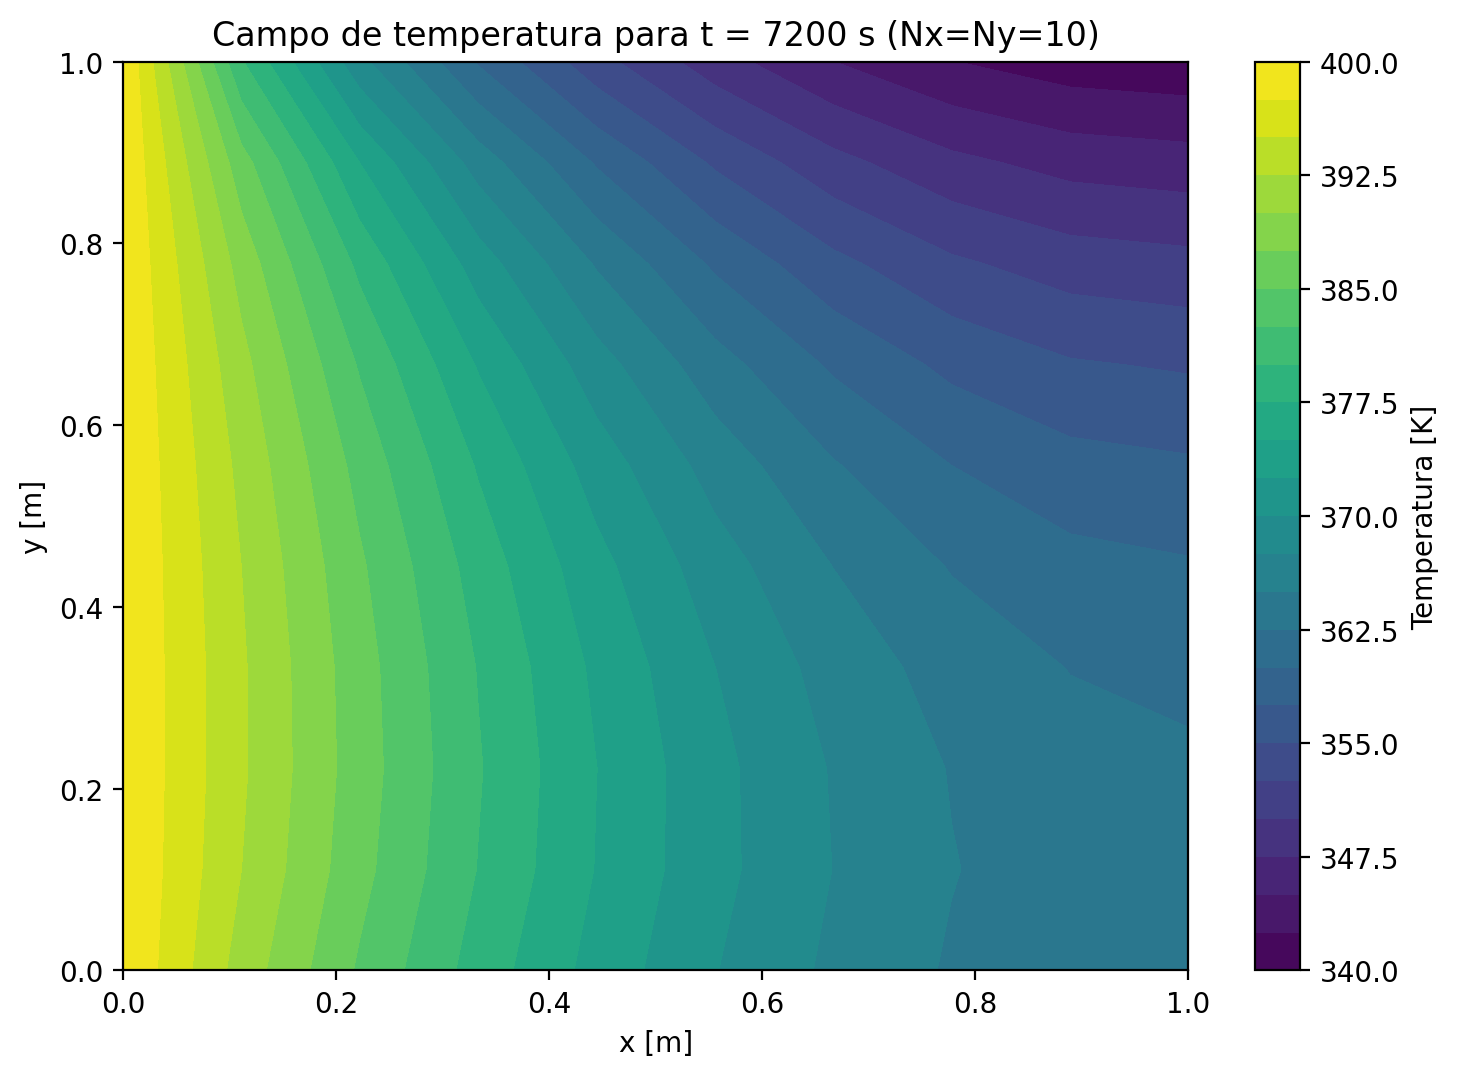
\includegraphics[width=0.75\textwidth]{figuras_avaliacao/campo_temperatura_t_07200.png}
    \caption{Campo de temperatura no instante $t=7200\ \text{s}$ para $N_x=N_y=10$.}
    \label{fig:campo_t7200}
\end{figure}

\begin{figure}[H]
    \centering
    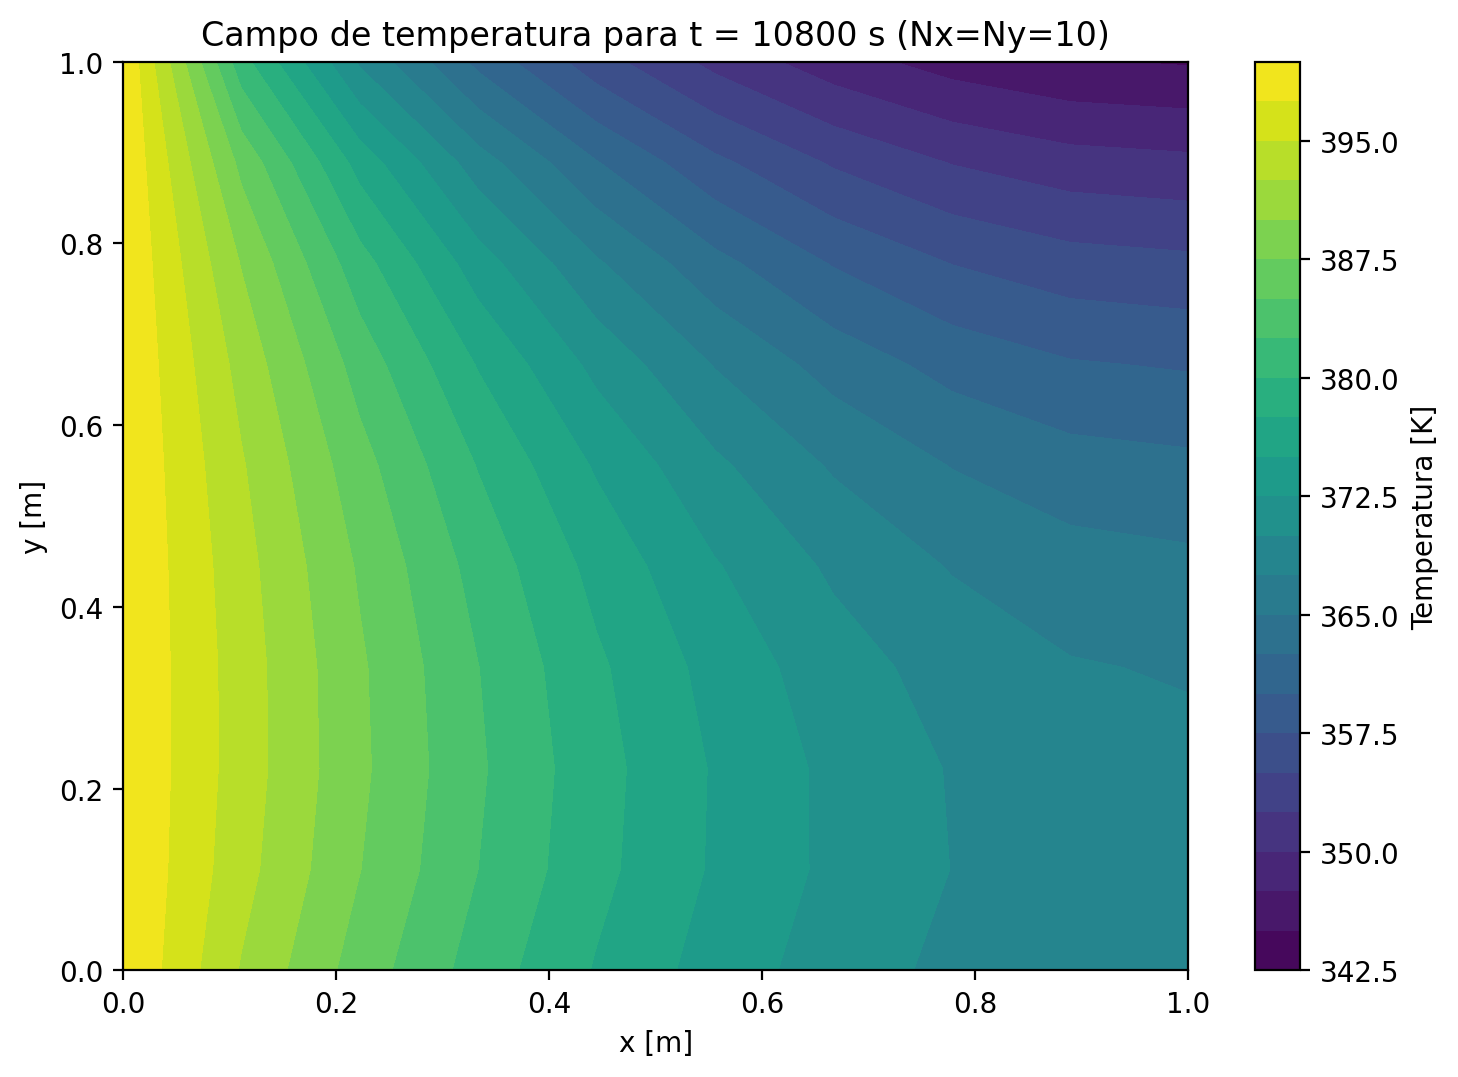
\includegraphics[width=0.75\textwidth]{figuras_avaliacao/campo_temperatura_t_10800.png}
    \caption{Campo de temperatura no instante $t=10800\ \text{s}$ para $N_x=N_y=10$.}
    \label{fig:campo_t10800}
\end{figure}

\begin{figure}[H]
    \centering
    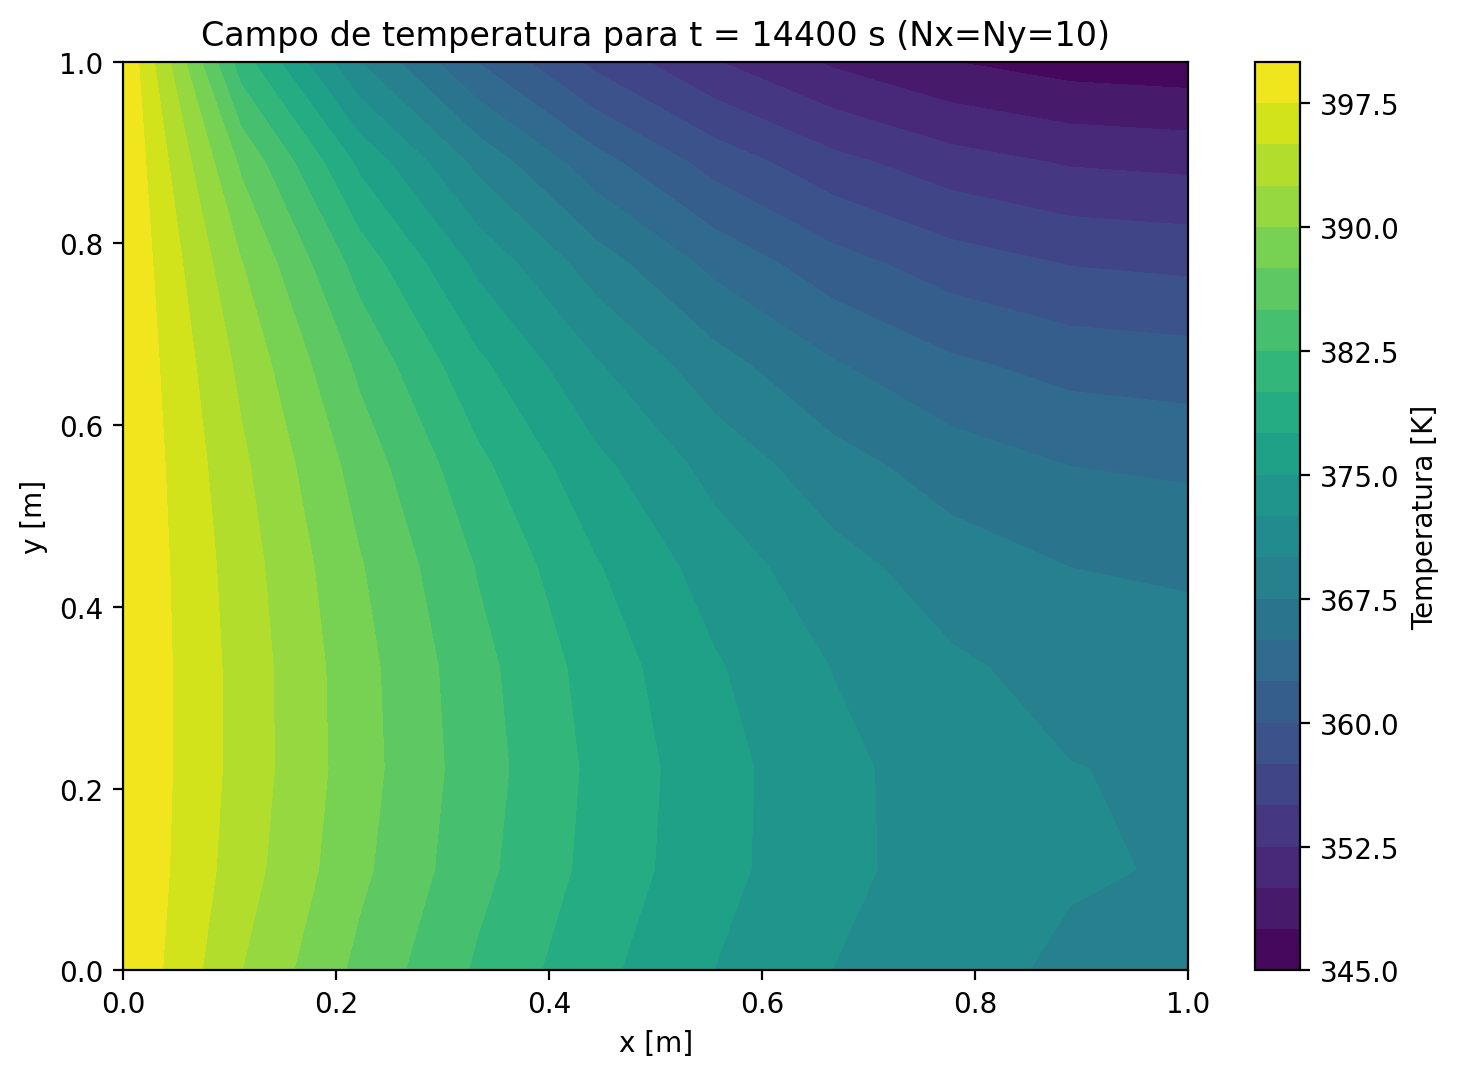
\includegraphics[width=0.75\textwidth]{figuras_avaliacao/campo_temperatura_t_14400.png}
    \caption{Campo de temperatura no instante $t=14400\ \text{s}$ para $N_x=N_y=10$.}
    \label{fig:campo_t14400}
\end{figure}

As Figuras~\ref{fig:campo_t0} a~\ref{fig:campo_t14400} mostram a evolução do campo térmico ao longo do tempo para a malha base solicitada no enunciado.

\subsection{Perfis de temperatura em $t=4\,$h}
\begin{figure}[H]
    \centering
    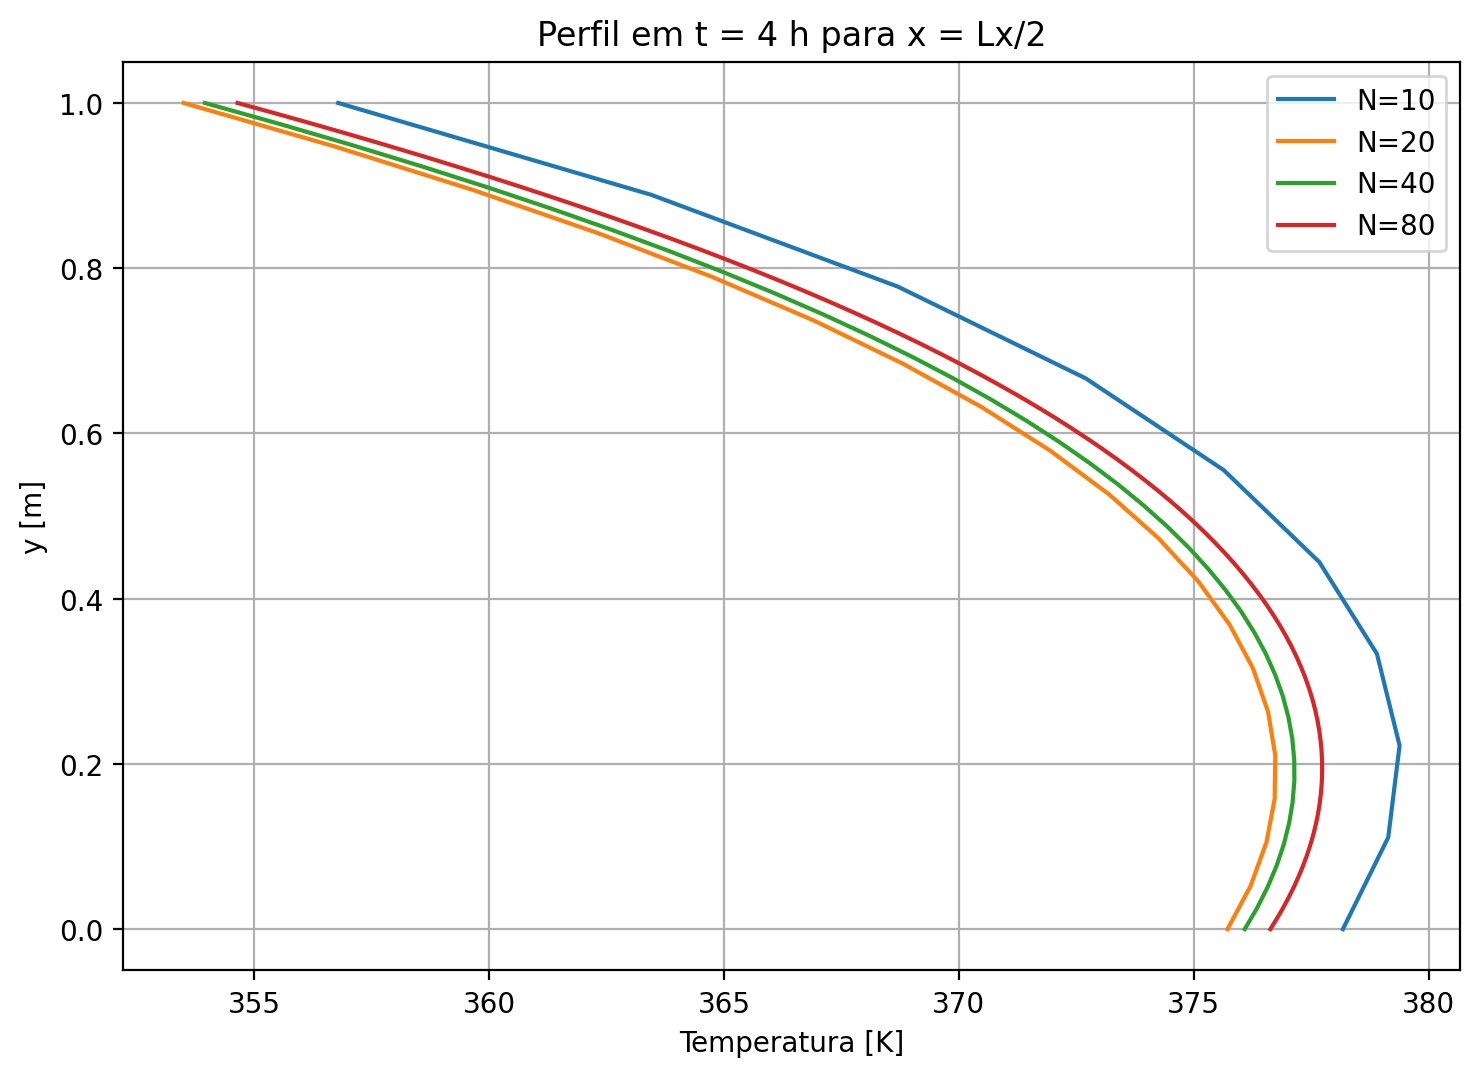
\includegraphics[width=0.75\textwidth]{figuras_avaliacao/perfil_x_meio.png}
    \caption{Perfil de temperatura em $t=4\,$h para $x=L_x/2$, comparando as malhas $10\times 10$, $20\times 20$, $40\times 40$ e $80\times 80$.}
    \label{fig:perfil_x_meio}
\end{figure}

\begin{figure}[H]
    \centering
    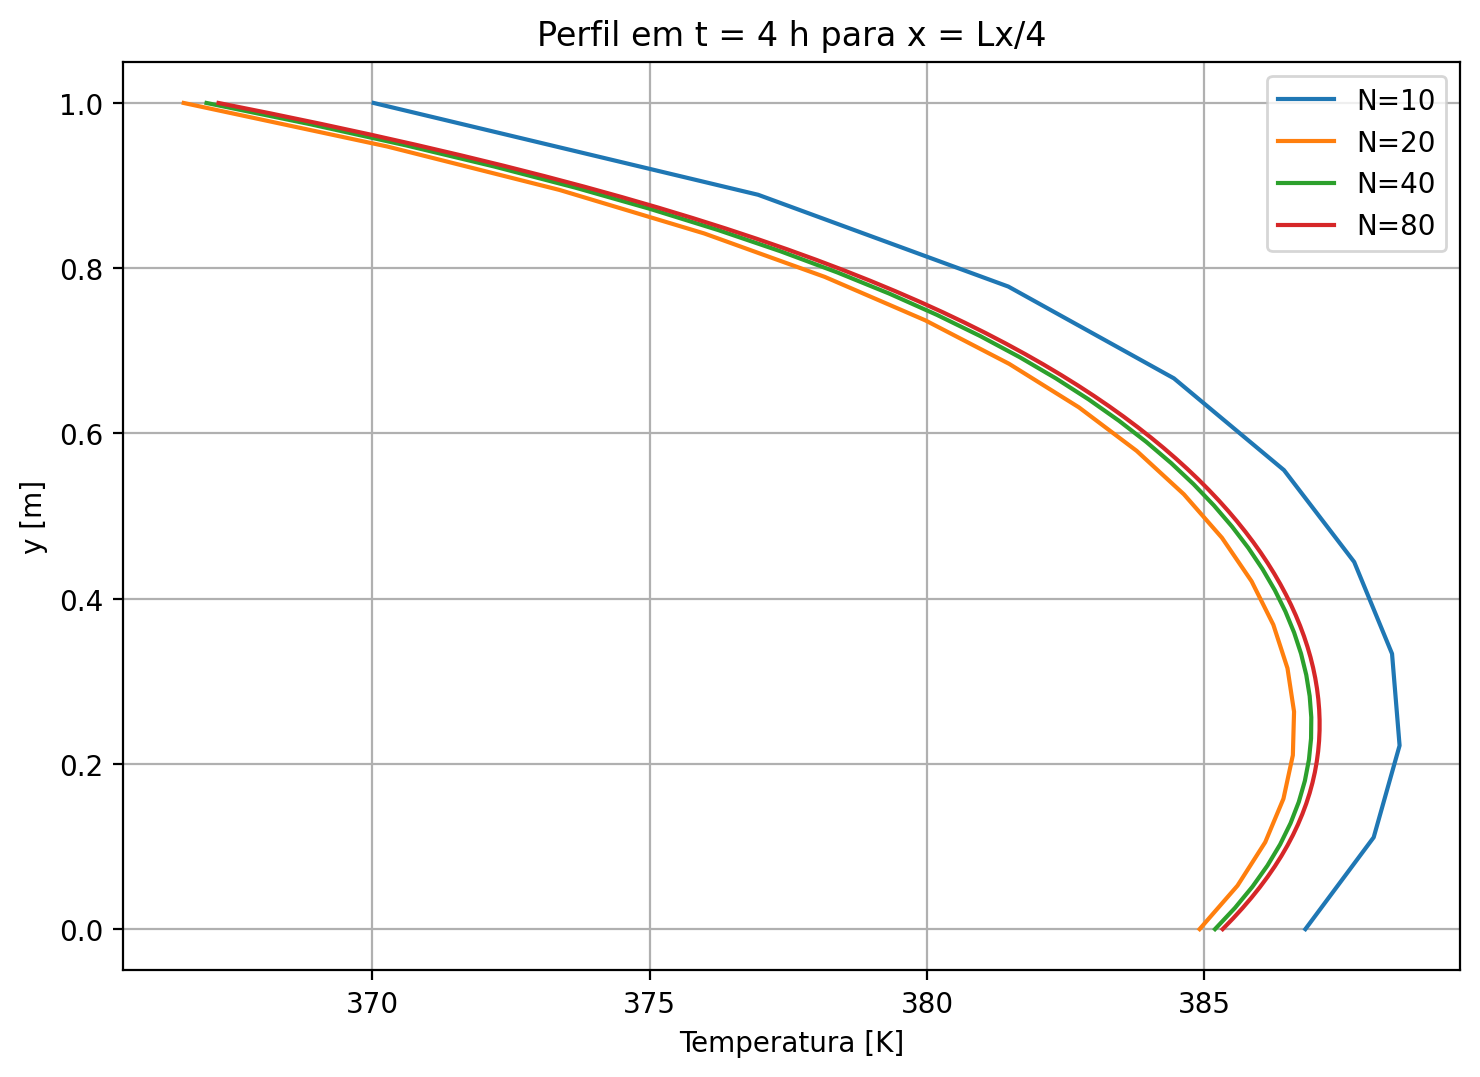
\includegraphics[width=0.75\textwidth]{figuras_avaliacao/perfil_x_quarto.png}
    \caption{Perfil de temperatura em $t=4\,$h para $x=L_x/4$, comparando as malhas $10\times 10$, $20\times 20$, $40\times 40$ e $80\times 80$.}
    \label{fig:perfil_x_quarto}
\end{figure}

\begin{figure}[H]
    \centering
    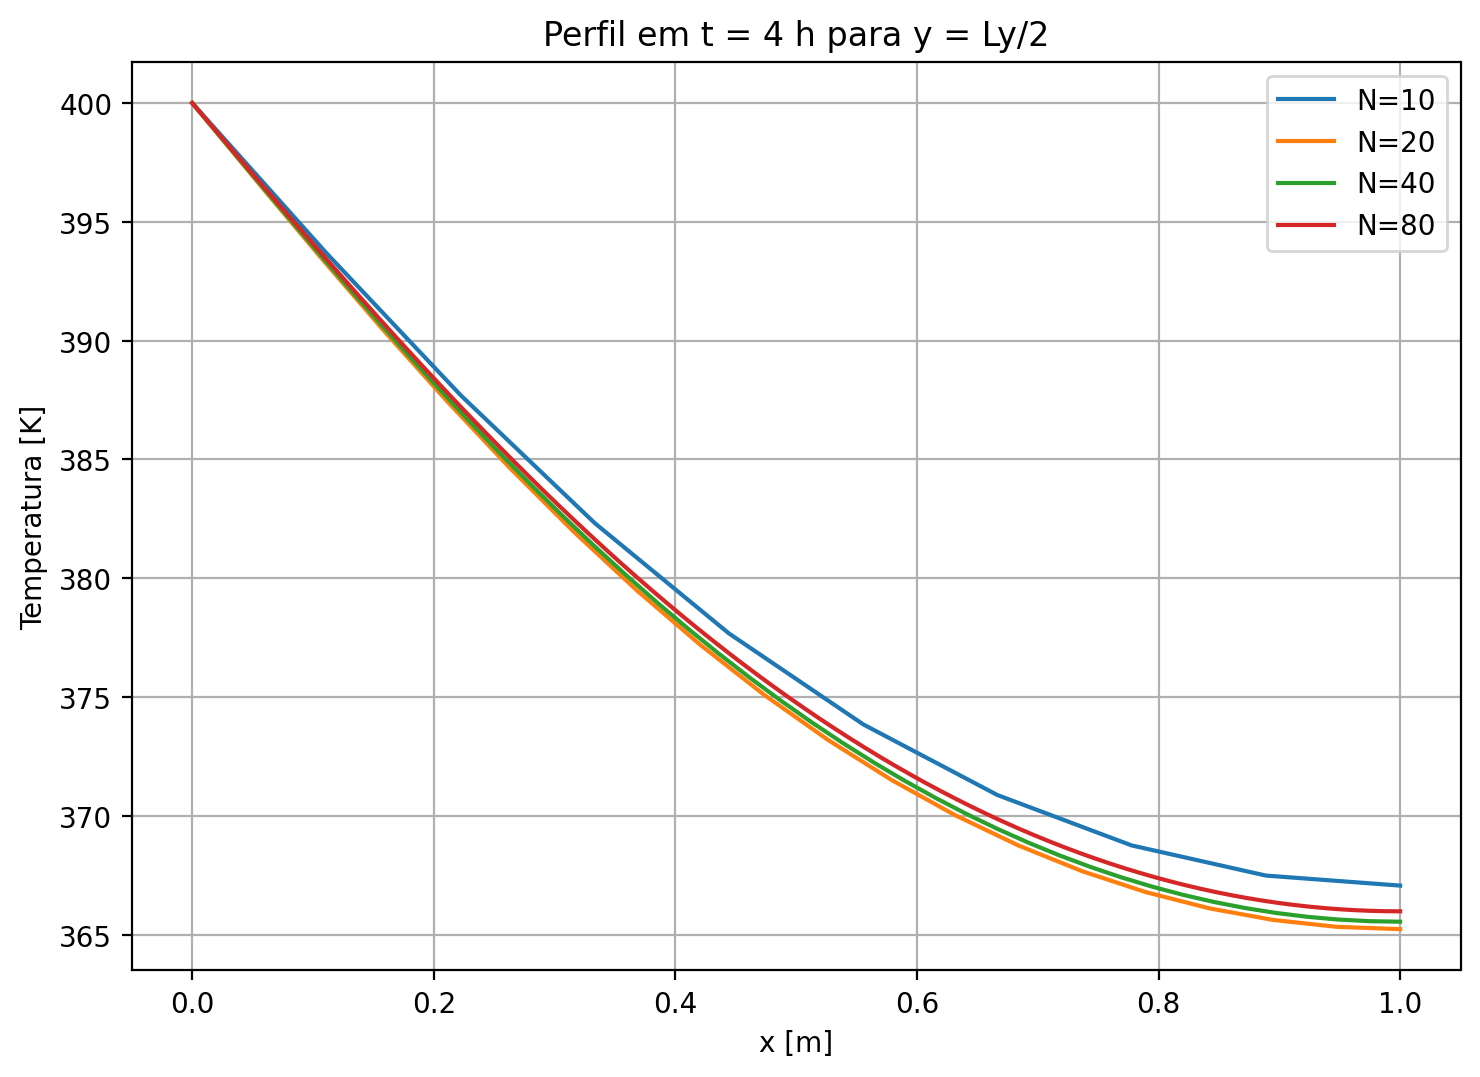
\includegraphics[width=0.75\textwidth]{figuras_avaliacao/perfil_y_meio.png}
    \caption{Perfil de temperatura em $t=4\,$h para $y=L_y/2$, comparando as malhas $10\times 10$, $20\times 20$, $40\times 40$ e $80\times 80$.}
    \label{fig:perfil_y_meio}
\end{figure}

\begin{figure}[H]
    \centering
    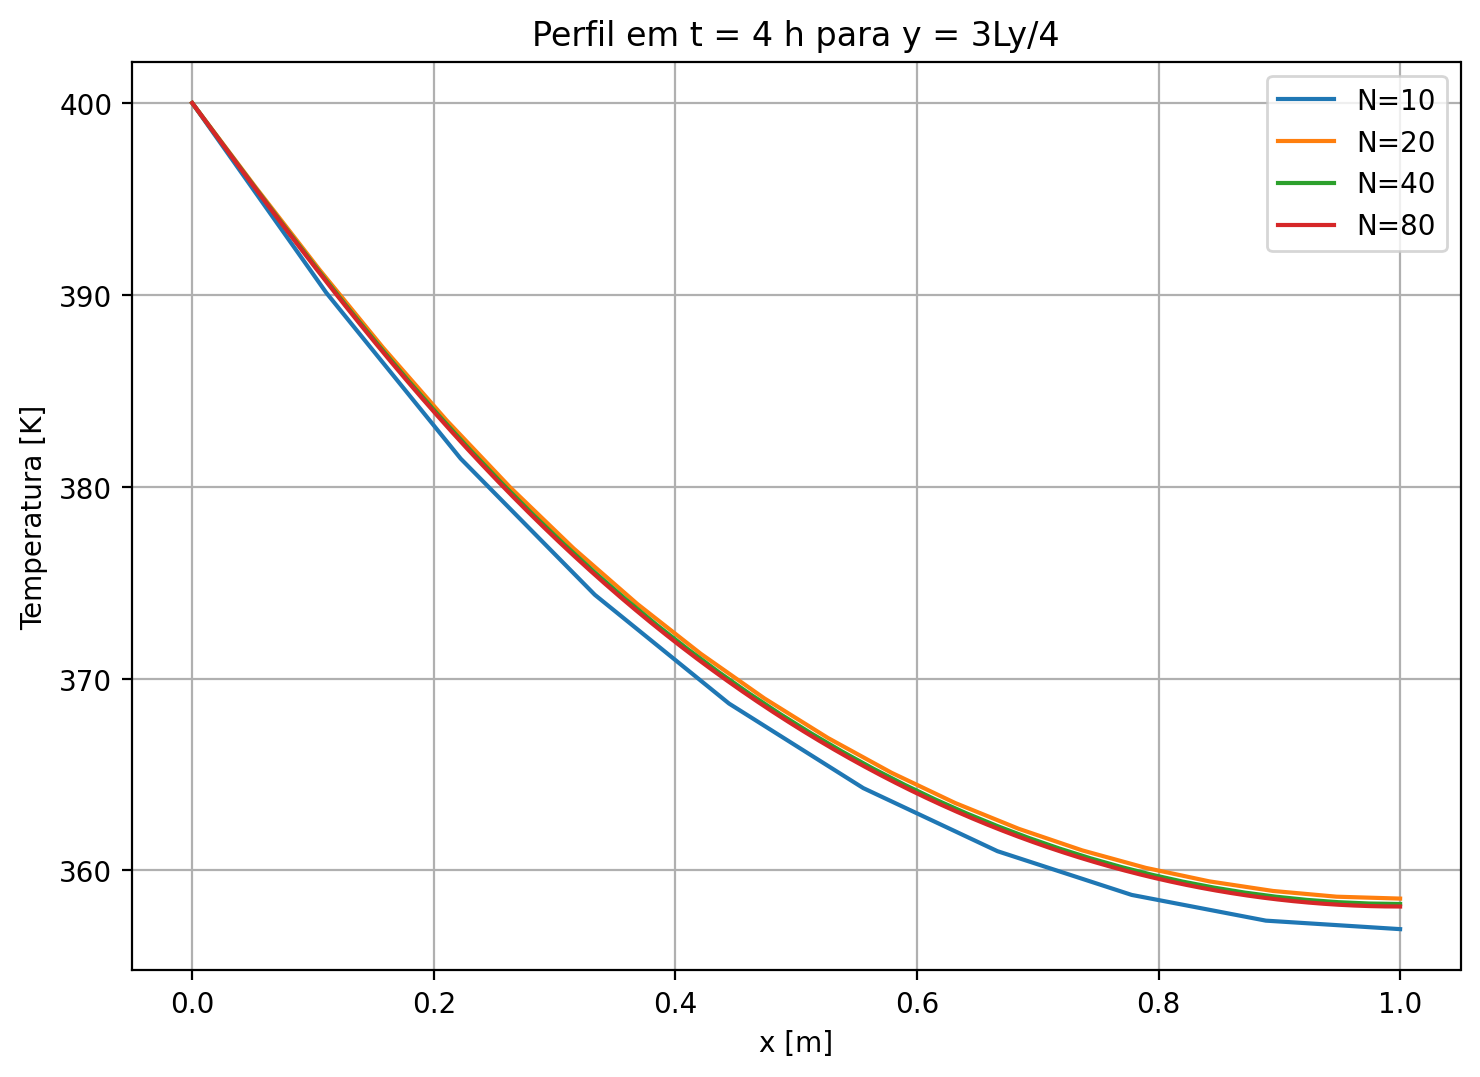
\includegraphics[width=0.75\textwidth]{figuras_avaliacao/perfil_y_tres_quartos.png}
    \caption{Perfil de temperatura em $t=4\,$h para $y=3L_y/4$, comparando as malhas $10\times 10$, $20\times 20$, $40\times 40$ e $80\times 80$.}
    \label{fig:perfil_y_tres_quartos}
\end{figure}

Os perfis das Figuras~\ref{fig:perfil_x_meio} a~\ref{fig:perfil_y_tres_quartos} permitem avaliar o efeito do refinamento de malha na solução numérica final.

\subsection{Evolução temporal da temperatura}
\begin{figure}[H]
    \centering
    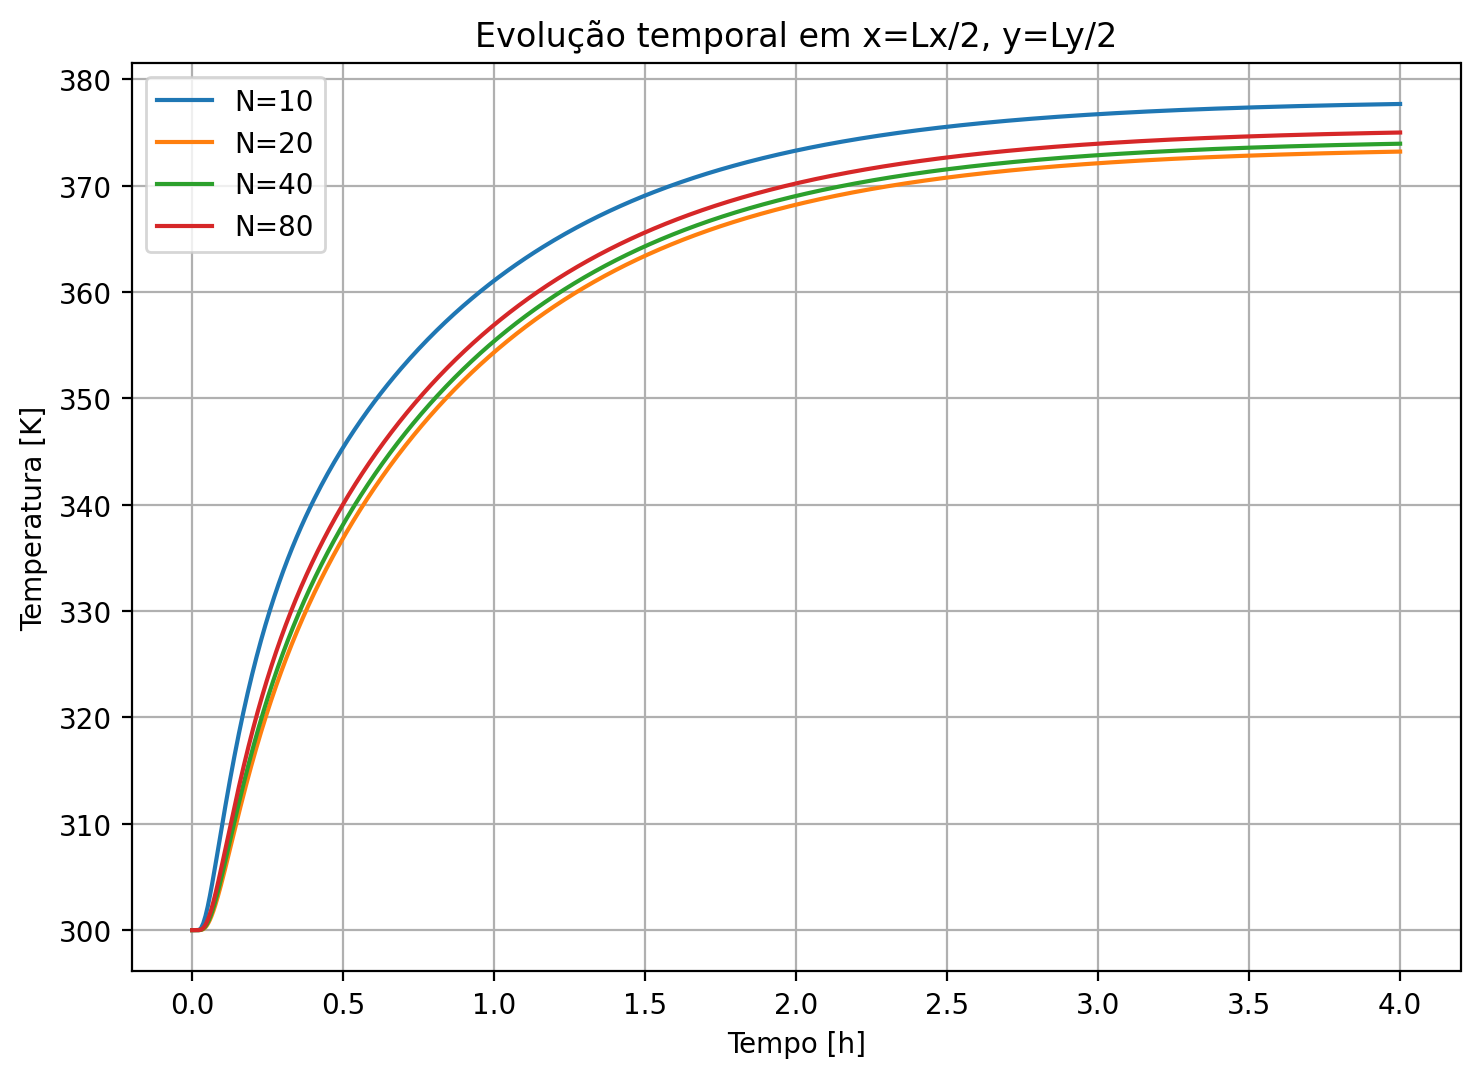
\includegraphics[width=0.75\textwidth]{figuras_avaliacao/historico_centro.png}
    \caption{Evolução temporal da temperatura em $x=L_x/2$ e $y=L_y/2$, comparando diferentes malhas.}
    \label{fig:historico_centro}
\end{figure}

\begin{figure}[H]
    \centering
    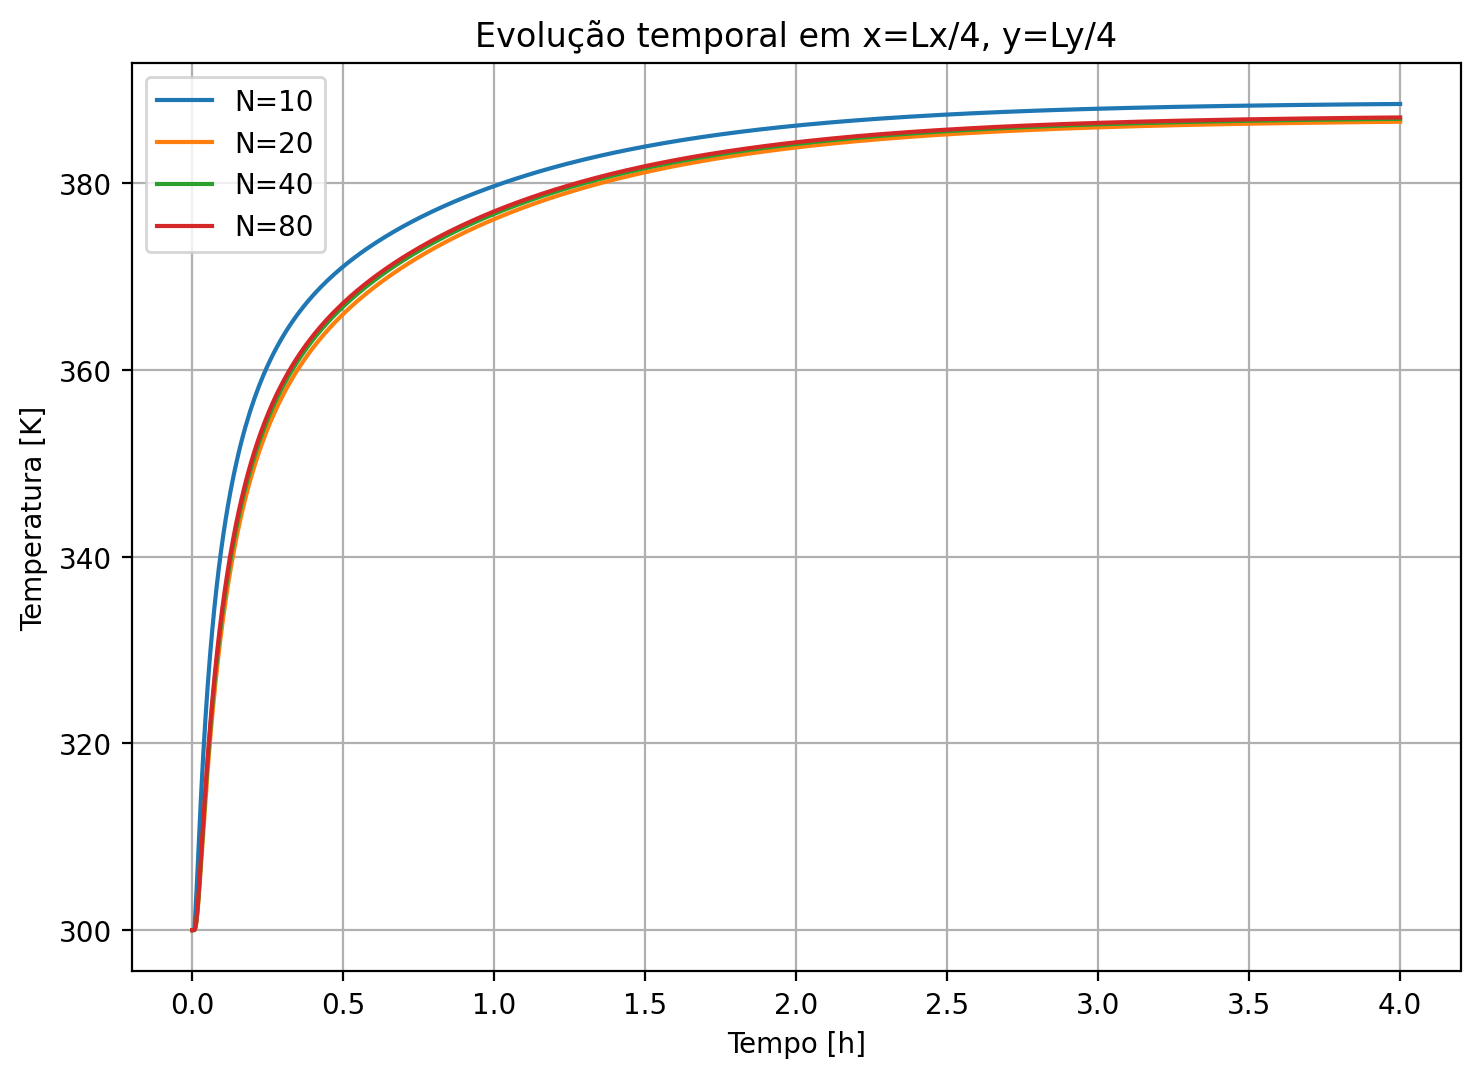
\includegraphics[width=0.75\textwidth]{figuras_avaliacao/historico_quarto.png}
    \caption{Evolução temporal da temperatura em $x=L_x/4$ e $y=L_y/4$, comparando diferentes malhas.}
    \label{fig:historico_quarto}
\end{figure}

As Figuras~\ref{fig:historico_centro} e~\ref{fig:historico_quarto} mostram como a temperatura evolui no tempo em pontos representativos do domínio, evidenciando a convergência entre malhas mais refinadas.

\section{Comentários finais}
O código apresentado atende diretamente ao que foi solicitado na avaliação: formulação da equação governante, discretização por diferenças finitas centrais de segunda ordem, integração temporal por Euler, implementação computacional, geração automática dos gráficos pedidos e comparação de diferentes malhas. Além disso, a implementação inclui suporte opcional a GPU com CUDA, mas mantém compatibilidade com execução serial em CPU quando a aceleração não estiver disponível.

\end{document}
